\documentclass[journal]{vgtc}                % final (journal style)
%\documentclass[review,journal]{vgtc}         % review (journal style)
%\documentclass[widereview]{vgtc}             % wide-spaced review
%\documentclass[preprint,journal]{vgtc}       % preprint (journal style)
%\documentclass[electronic,journal]{vgtc}     % electronic version, journal

%% Uncomment one of the lines above depending on where your paper is
%% in the conference process. ``review'' and ``widereview'' are for review
%% submission, ``preprint'' is for pre-publication, and the final version
%% doesn't use a specific qualifier. Further, ``electronic'' includes
%% hyperreferences for more convenient online viewing.

%% Please use one of the ``review'' options in combination with the
%% assigned online id (see below) ONLY if your paper uses a double blind
%% review process. Some conferences, like IEEE Vis and InfoVis, have NOT
%% in the past.

%% Please note that the use of figures other than the optional teaser is not permitted on the first page
%% of the journal version.  Figures should begin on the second page and be
%% in CMYK or Grey scale format, otherwise, colour shifting may occur
%% during the printing process.  Papers submitted with figures other than the optional teaser on the
%% first page will be refused.

%% These three lines bring in essential packages: ``mathptmx'' for Type 1
%% typefaces, ``graphicx'' for inclusion of EPS figures. and ``times''
%% for proper handling of the times font family.

\usepackage{mathptmx}
\usepackage{graphicx}
\usepackage{times}
\usepackage{balance}
\usepackage{appendix}
\usepackage{verbatim}
\usepackage[nooneline,hang,it,IT]{subfigure}

%% We encourage the use of mathptmx for consistent usage of times font
%% throughout the proceedings. However, if you encounter conflicts
%% with other math-related packages, you may want to disable it.

%% This turns references into clickable hyperlinks.
\usepackage[bookmarks,backref=true,linkcolor=black]{hyperref} %,colorlinks
\hypersetup{
  pdfauthor = {},
  pdftitle = {},
  pdfsubject = {},
  pdfkeywords = {},
  colorlinks=true,
  linkcolor= black,
  citecolor= black,
  pageanchor=true,
  urlcolor = black,
  plainpages = false,
  linktocpage
}

%% If you are submitting a paper to a conference for review with a double
%% blind reviewing process, please replace the value ``0'' below with your
%% OnlineID. Otherwise, you may safely leave it at ``0''.
\onlineid{0}

%% declare the category of your paper, only shown in review mode
\vgtccategory{Research}

%% allow for this line if you want the electronic option to work properly
\vgtcinsertpkg

%% In preprint mode you may define your own headline.
%\preprinttext{To appear in an IEEE VGTC sponsored conference.}

%% Paper title.

\title{Analytics of the Dino Fun Crime problem}

%% This is how authors are specified in the journal style

%% indicate IEEE Member or Student Member in form indicated below
\author{Carl Englund, Einar Sandberg, Klas Eskilson}


%% Abstract section.
\abstract{This report is written for a data analytics project in the course TNM098 (Advance Visual Data Analysis) at Linköpings University. It covers the development process of data mining techniques and visualization of a data set covering a amusement park over a weekend.}
%% Keywords that describe your work. Will show as 'Index Terms' in journal
%% please capitalize first letter and insert punctuation after last keyword
\keywords{Multivariate data}



%%%%%%%%%%%%%%%%%%%%%%%%%%%%%%%%%%%%%%%%%%%%%%%%%%%%%%%%%%%%%%%%
%%%%%%%%%%%%%%%%%%%%%% START OF THE PAPER %%%%%%%%%%%%%%%%%%%%%%
%%%%%%%%%%%%%%%%%%%%%%%%%%%%%%%%%%%%%%%%%%%%%%%%%%%%%%%%%%%%%%%%%

\begin{document}

%% The ``\maketitle'' command must be the first command after the
%% ``\begin{document}'' command. It prepares and prints the title block.

%% the only exception to this rule is the \firstsection command
\firstsection{Introduction}

\maketitle The report covers the implementation of algorithms and techniques used to uncover anomalies in a large dataset, as well as how to make the data run effectively even though the large size of the dataset. 

The task at hand was to determine when the crime introduced in a news article attached to the data set used occured. Issues that will be discussed will be the following:
\begin{itemize}
	\item When did the crime occur?
	\item Is it possible to determine who or whom committed the crime?
	\item Did the crime affect the park in any way more than a partial closure during the time of the event?	
\end{itemize}

\section{Data}
The used dataset for this project was retrieved from the Mini-challenge of VAST\footnote{Visual Analytics Community
} Challenge 2015. The dataset is from a theme park, and contains information about each visitors movement. It was stored in three CSV-files\footnote{Comma-separated value
} each representing a single day of a weekend. Every file had five datums representing, a timestamp,  an ID of a single person, an activity of either a movement or a check-in as well as two coordinates, X and Y. See table \ref{dataexample} for an typical line of data in the files.

As persons move through the park their movements are recorded with a one-second resolution. If the user does not get an new coordinate each second it means that they have not moved out of their current grid area. Each grid area is 5x5 meters and the entire park spans over 250 000 square meters.

\begin{table}[h!]
\centering
\caption{Example data}
\label{dataexample}
\begin{tabular}{|l|l|l|l|l|}
\hline
\textbf{Timestamp} & \textbf{id} & \textbf{Type} & \textbf{X} & \textbf{Y} \\ \hline
2014-6-07 08:00:08 & 1102394     & check-in      & 99         & 77         \\ \hline
2014-6-07 08:00:08 & 1187304     & check-in      & 63         & 99         \\ \hline
2014-6-07 08:00:08 & 1363700     & check-in      & 99         & 77         \\ \hline
2014-6-07 08:00:10 & 1449032     & check-in      & 63         & 99         \\ \hline
2014-6-07 08:00:10 & 279658      & check-in      & 63         & 99         \\ \hline
2014-6-07 08:00:27 & 657863      & movement      & 7          & 43         \\ \hline
2014-6-07 08:00:35 & 657863      & movement      & 8          & 43         \\ \hline
\end{tabular}
\end{table}
Since the recordings were at a one-second resolution each file contained a rather large amount of data. The three given files contained data for three different days. Its timespace was roughly between 08.00 to around 23.30 every day, with logs every second if a visitor’s position had changed. In order to reduce this to a reasonable amount, algorithms and deletion of redundant data was used as described further on in the report.


\section{Method}
Several different methods were used in order to interpret the data, both visually and analytically. Initially, a Java application with the ability to convert the data to separate visitors was created. Every separate visitor contained information about the time and location of the visitor’s movement.

The application was then extended with functionality to process the data into a new CSV-file, containing coordinates and the amount of people having visited those coordinates. These coordinates were grouped by time a time period of a given length, for instance 10:05 to 10:10. From this CSV-file, D3.js was used to create a simple web application containing a heat map which shows the intensity in which different places on the map have been visited. The user were able to select what time period it wanted to see using a simple slider. This allowed the user to visually analyze the flow of the park visitors’ movements throughout the day.

Functionality to categorize the visitors into groups, based on their movement patterns was also developed. If two visitors have visited the same coordinate the same minute a thousand times, they’re seen as part of the same group. The program also calculated when groups of visitors created anomalies in the movement flow throughout the park for each 10-minute period, much like what was done visually with the heat map. This method also supported printing of information regarding anomalies around certain points of interest, for example the Creighton Pavilion. The program then printed what large flow change (relative to the mean change for each coordinate) was found around these points. 

The application was also extended with methods to analyze separate visitors’ movement. By analyzing each visitors movement, and calculating the mean time between the logged locations, the program could detect when a person was standing still for a unusual long time. The application also summed each separate visitor’s total waiting time.


\section{Results}
The analytical method for finding anomalies in the visitor flow throughout the park was mainly targeted around Creighton Pavilion. This is where the crime was assumed to have taken place, since the given background information about the crime indicated this. Therefore, anomalies within the square given by the points (20, 20) and (40, 40) was printed. The points that were found is in Appendix A, where the change is the difference between the previous amount of people at a given coordinate and the current amount of people at that coordinate.

The visualization implemented consists of a scatter plot with the map of the park as a background. In the scatter plot, visits at coordinates over a certain time is shown. At the moment it is possible to display where people have been in a 5 minute timespan. See figure \ref{fig:pc}. In this figure different positions of where people were been at 10.50 to 10.55AM on Sunday can be seen. The stronger the color of the red dot the more people have been logged at that position.

\begin{figure}[h!]
  \begin{center}
    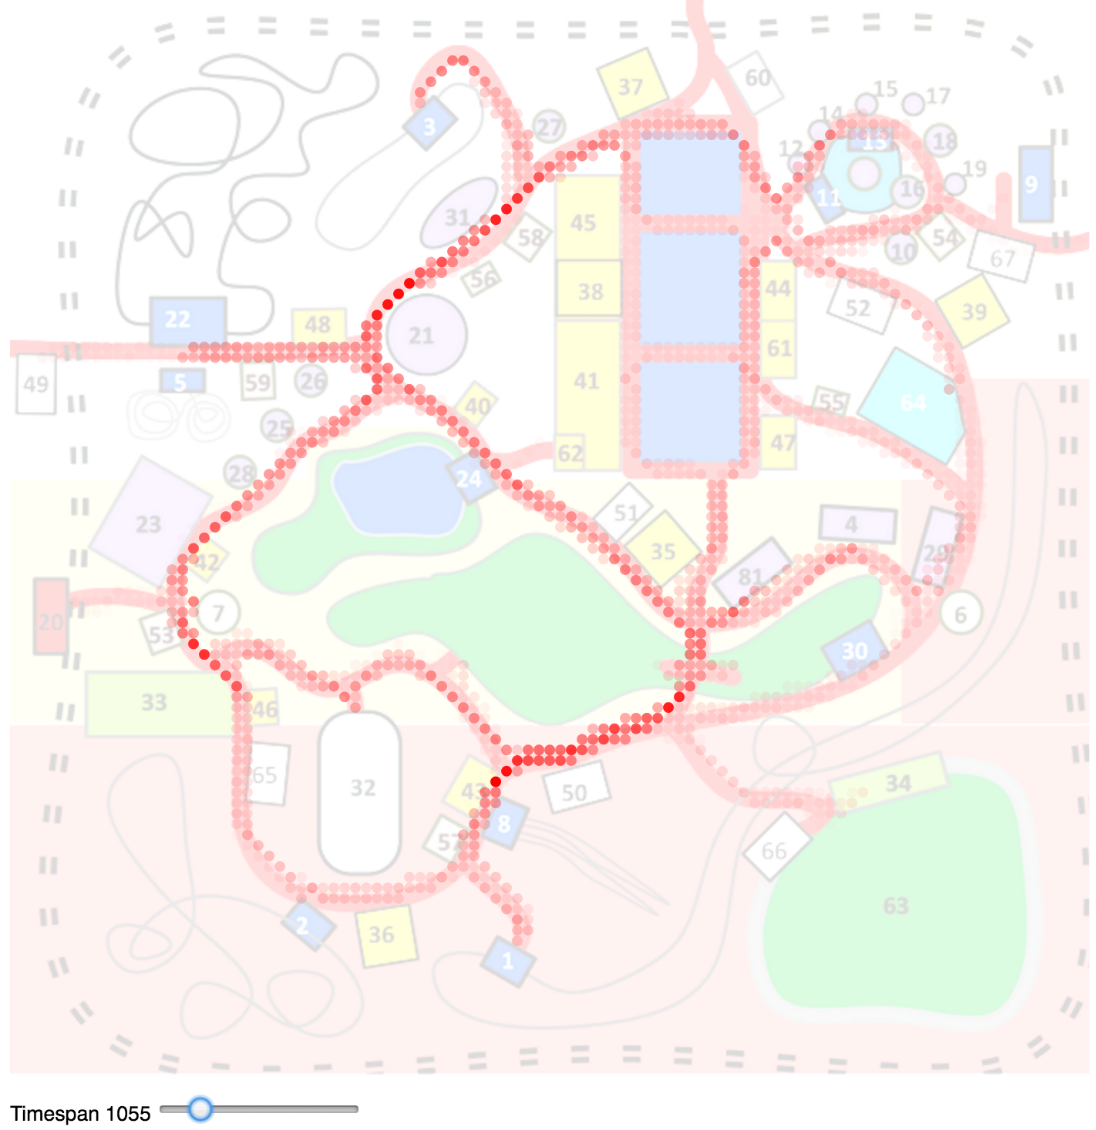
\includegraphics[scale=0.4]{img/pic.png}
    \caption{\label{fig:pc}The visual application}

  \end{center}
\end{figure}

The feature for categorizing visitors into groups produced a text file with groups containing  the visitor ID:s. In the current implementation, a number of visitors is considered a group if they share the same coordinates at the same timestamp (with an accuracy of minutes) a thousand times. However, it It is possible to specify how to categorize these groups. For example, if one would want more precise grouping, the required amount of shared coordinates could be increased, or one could use a more narrow timestamp accuracy. Using the produced text file could help you draw conclusion about suspected visitors. See attached text file for produced result.

The program’s ability to detect if a visitor was standing still for an extended time period produced a lot of data; too large to attach to this report in a sane way. For example, the file containing movement data for the sunday found 1512 visitors having a total waiting time over 50000 seconds.


\section{Discussion}
Given the nature of the task, it was not possible trying to filter the initial data which would allow us to work with a more reasonable amount of data. This proved to be a challenge for the project, since the goal was to find anomalies in the data in order to get more information about the event at Creighton Pavilion. All visitors were of interest, and therefore none of the initial data could be removed or filtered out. Consequently, many of the algorithms proved to be time consuming, which eliminated the option of effectively testing the algorithms for optimal parameter values.

Since the data size is very large, the algorithm for categorizing visitors into groups were really time consuming, which means testing the algorithm and trying to find the optimal values for the different parameters were impossible. It’s hard to know what should be interpreted as a group without varying the time accuracy and amount of equal coordinates, and comparing the results to the initial data to see if the groups are plausible.

The visual application was limited to displaying visitors and their positions over the last five minutes. The timespan was generated through the Java program and it could be time consuming if the timespan would be changed to more than or less than five minutes. This is something that could be further developed to make it easier to visually analyze the data.

While the program were able to detect persons standing still for an extended time period, the use of the result turned out to be limited. The vast amount of data was, once again, a constraining factor. The program found a lot of visitors standing still, but the result was hard to interpret and reduce to a comprehensible extent. Here, a visual representation might have been of use to make it easier to understand where these visitors moved. Instead of viewing all visitors from the entire data set, a smaller subset containing the stationary visitors might have been easier to comprehend and make use of.

The flow anomaly analysing method gave some interesting results. There are large differences between the amount of anomalies found on the Sunday compared to both the Friday and Saturday. This may be an indication that the Sunday is more interesting than the other days, since according to the given news article, the park was partially closed after the crime.

Although the flow analysing method gave results, it could have been improved further. The parameters that control how the data is reduced, how large the area that the method analyses were and what time span the method uses, could benefit from being applicable in a more interactive manner. In the current state of the application, these are constants set before compilation. This limits the way these variables could be used to further understand the data. However, since the amount of data is vast, in order to actually achieve interactivity with acceptable performance, this would require that the data is reduced before the methods are applied. This poses another challenge that have not yet been tackled – data reduction.

Moreover, the flow anomaly detection could perhaps have been improved by another mathematical method than the mean which was used. Standard deviation, or similar statistical methods could have been tested to see if they would produce a more distinct result.

Something that should have been focused more on in the project is to combine the different methods used. As of now there is a number of different methods used, but none of them use each other's results. If two methods were combined it might provide more insight into the initial questions asked and the answer to them.

Furthermore, to make it easier to analyse the data, other visual tools could have been used. In the application, there was only one visual method implemented – the heat map. To further understand how occupied a certain area was during a park, line charts or other similar methods could have been applied. This could help an analyst to quickly identify any irregularities in how people moved, for instance. Then, a more precise time and place for the crime could perhaps have been found.


\section{Conclusion}
While some vague indications that the Sunday may be more interesting were given by the results, it has not been possible to narrow down the time more precisely. From the result, it has neither been possible to determine who committed the crime, as no unique visitor stood out notably. Neither have any conclusion been drawn regarding the effect the event had on the park’s openings.

\appendix
\onecolumn
\chapter{The first appendix} 


\begin{table}[]
\centering
\caption{My caption}
\label{my-label}
\begin{tabular}{|l|l|l|l|l|l|}
\hline
File name & File size & Number of lines & Start time & End time & Unique visitors \\ \hline
\begin{tabular}[c]{@{}l@{}}park-movement-\\ Fri.csv\end{tabular} & 238 MB & 6 010 915 & \begin{tabular}[c]{@{}l@{}}2014-06-06\\ 08:00:16\end{tabular} & \begin{tabular}[c]{@{}l@{}}2014-06-06\\ 23:26:36\end{tabular} & 3557 \\ \hline
\begin{tabular}[c]{@{}l@{}}park-movement-\\ Sat.csv\end{tabular} & 359 MB & 9 078 624 & \begin{tabular}[c]{@{}l@{}}2014-06-07\\ 08:00:08\end{tabular} & \begin{tabular}[c]{@{}l@{}}2014-06-07\\ 23:35:24\end{tabular} & 6411 \\ \hline
\begin{tabular}[c]{@{}l@{}}park-movement-\\ Sun.csv\end{tabular} & 432 MB & 10 932 426 & \begin{tabular}[c]{@{}l@{}}2014-06-08\\ 08:00:11\end{tabular} & \begin{tabular}[c]{@{}l@{}}2014-06-08\\ 23:25:13\end{tabular} & 7659 \\ \hline
\end{tabular}
\end{table}

\end{document}


